\documentclass[a4paper,12pt]{article} 
\usepackage[T2A]{fontenc}			
\usepackage[utf8]{inputenc}			
\usepackage[english,russian]{babel}
\usepackage{float}
\usepackage{amsmath,amsfonts,amssymb,amsthm,mathrsfs,mathtools} 
\usepackage{cancel}
\usepackage{multirow}
\usepackage[colorlinks, linkcolor = blue]{hyperref}
\usepackage{upgreek}\usepackage[left=2cm,right=2cm,top=2cm,bottom=3cm,bindingoffset=0cm]{geometry}
\usepackage{tikz}
\usepackage{graphicx}
\usepackage{subfig}
\usepackage{titletoc}
\usepackage{pgfplots}
\usepackage{xcolor}
\usepackage{wrapfig}
\usepackage{pgfplots}
\pgfplotsset{width=10cm,compat=1.9}

\begin{document}

\title{Лабораторная работа №4.4.2\\
<<Изучение призмы с помощью гониометра>>}

\author{Котова Александра, Чекмарев Игорь}

\maketitle
\textbf{Цель:} Знакомство с работой гониометра, исследование дисперсии стеклянной призмы и определение характеристик призмы как спектрального прибора.

\textbf{Оборудование:} Гониометр, ртутная лампа, призма, стеклянная плоскопараллельная пластинка, призменный уголковый отражатель.

\section{Гониометр}

Все измерения в данной работе производятся с помощью гониометра, он служит для точного измерения углов.

\begin{figure}[h!]
    \centering
    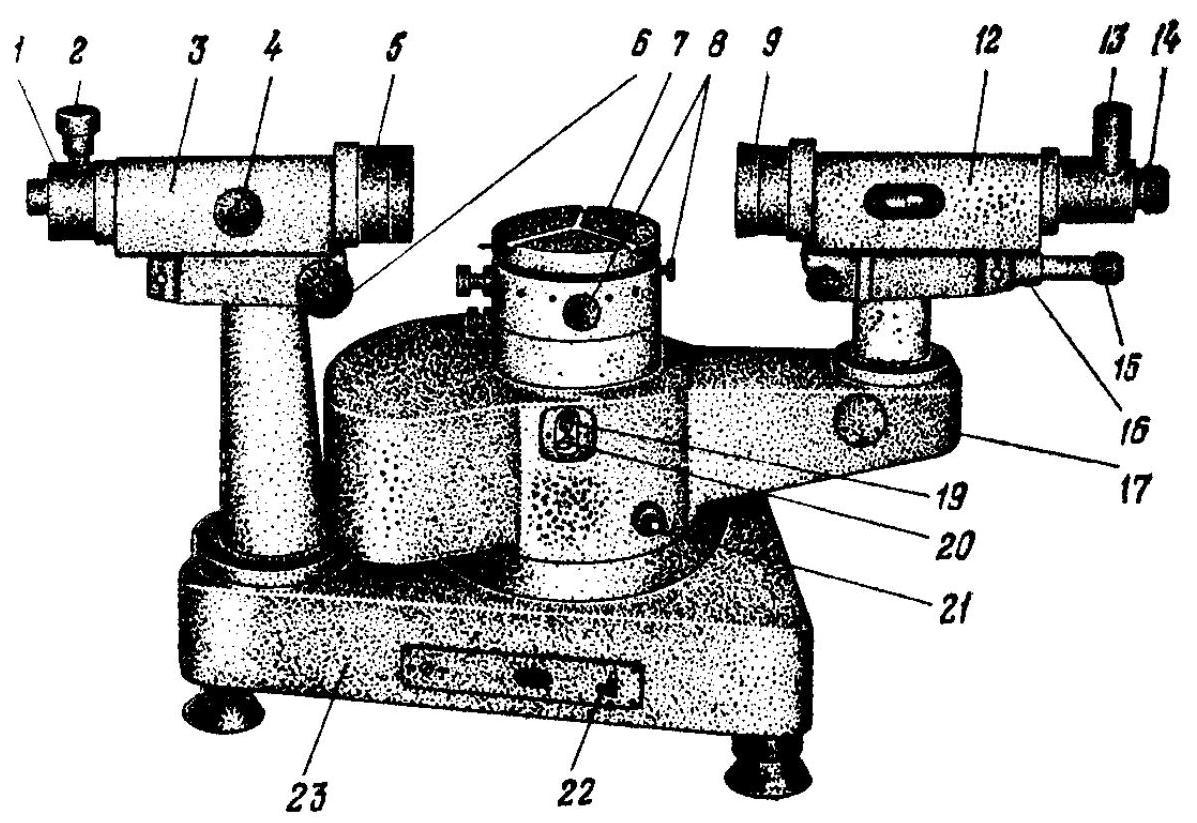
\includegraphics[width=0.5\linewidth]{2023_04_02_a48ae02e429ba186bcd7g-2(2).jpg}
    \caption{Устройство гониометра}
    \label{fig:placeholder}
\end{figure}



\section*{Теоретическая справка}

Гониометр используется для точного определения углов, а значит с его помощью можно точно определять показатели преломления и преломляющие угла призм и кристаллов, измерять длины волн спектральных линий и прочее. Например, показатель преломления удобно определять по углу наименьшего отклонения. При это показатель преломления определяется формулой

\begin{equation}
    n = \frac{\sin \frac{\alpha + \delta}{2}}{\sin \frac{\alpha}{2}},
\end{equation}

\noindent
где $\alpha$ -- преломляющий угол призмы, $\delta$ -- угол минимального отклонения, $n$ -- показатель преломления. \\

\section*{Ход работы}

\paragraph{Юстриовка гониометра} настроили зрительную трубу, предметный столик, коллиматор, входную щель, начало отсчета. В общем, настроили все, что смогли. При этом ноль отсчета углов составляет $182^\circ5'53''$. Установили призму.

\paragraph{Измерение преломляющего угла} для этого установим трубу последовательно перпегдикулярно обеим преломляющим гранями призмы, измерив углы, соответствующие этим положениям ($120^\circ40'0''$ и $237^\circ42'10''$). По ним можем определить преломляющий угол призмы $\alpha = 62^\circ57'50''$.

\paragraph{Минимальный угол отклонения} для этого снача найдем спектр, получаемый с помощью призмы. Затем настроим на него зрительную трубу и измерим минимум отклонения для каждой из спектральных линий. Результаты занесем в табл. 1.

\begin{table}[H]
    \centering
    \caption{Координаты спектральных линий}
    \begin{tabular}{|c|c|c|c|c|} \hline
         № & 1 & 2 & 3 & 4 \\ \hline
         $\delta$ & $128^\circ14'05''$ & $127^\circ34'05''$ & $126^\circ58'42''$ & $126^\circ56'49''$ \\ \hline
    \end{tabular}

    \vspace{0.5cm} % небольшой отступ между таблицами

    \begin{tabular}{|c|c|c|c|c|} \hline
         № & 5 & 6 & 7 & 8 \\ \hline
         $\delta$ & $126^\circ25'30''$ & $125^\circ09'55''$ & $123^\circ04'55''$ & $121^\circ12'50''$ \\ \hline
    \end{tabular}
\end{table}

\noindent
Пользуясь формулой (1), рассчитаем показатели преломления $n$ для всех значений угла из табл. 1. Результаты представлены в табл. 2.

\begin{figure}[h!]
    \centering
    \begin{minipage}{0.48\linewidth}
        \centering
        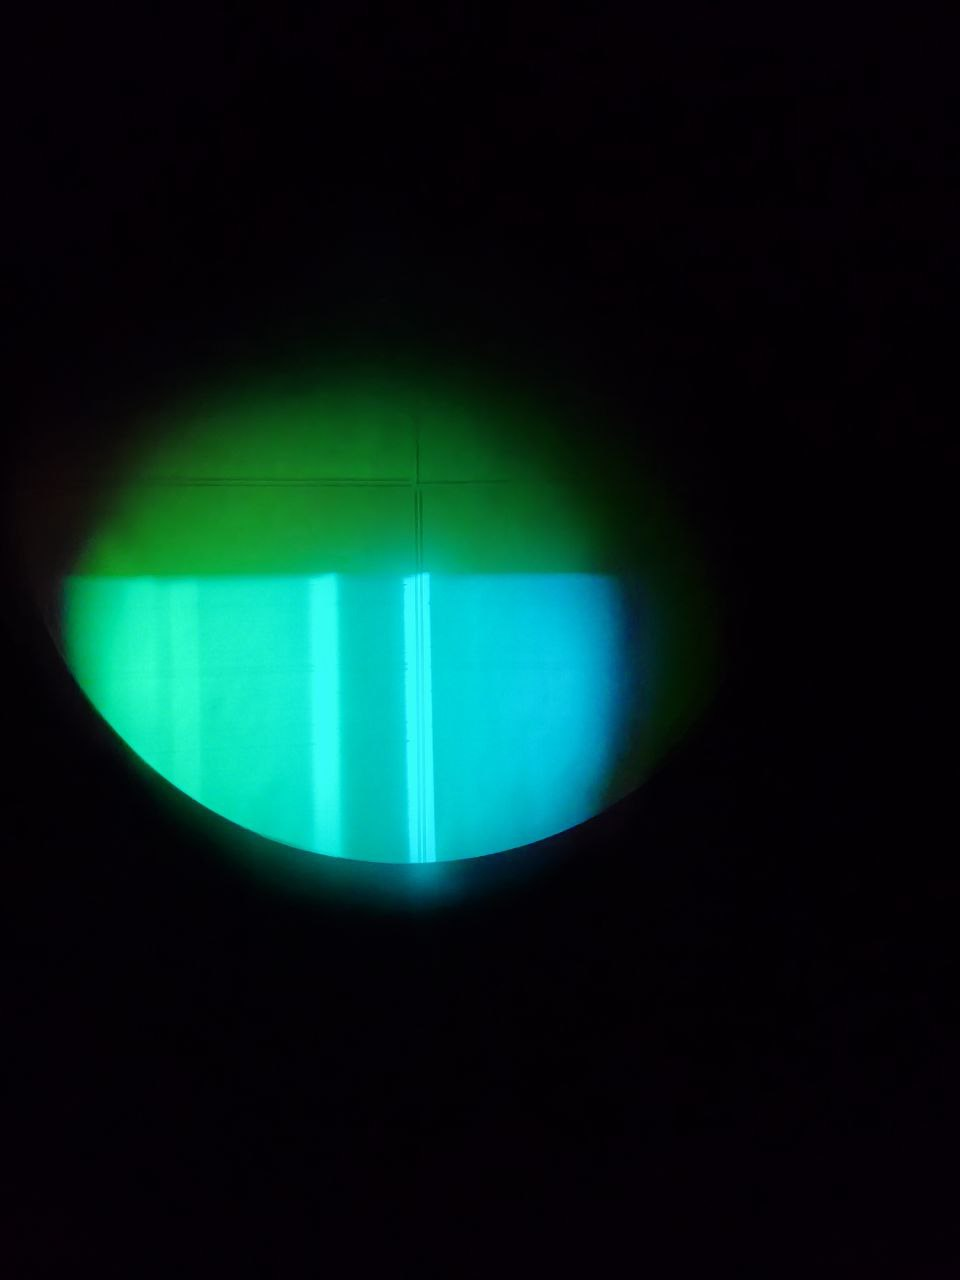
\includegraphics[width=\linewidth]{blue_specter.jpg}
        \caption{Часть спектра, свет длиной ~492 нм}
        \label{fig:placeholder}
    \end{minipage}
    \hfill
    \begin{minipage}{0.48\linewidth}
        \centering
        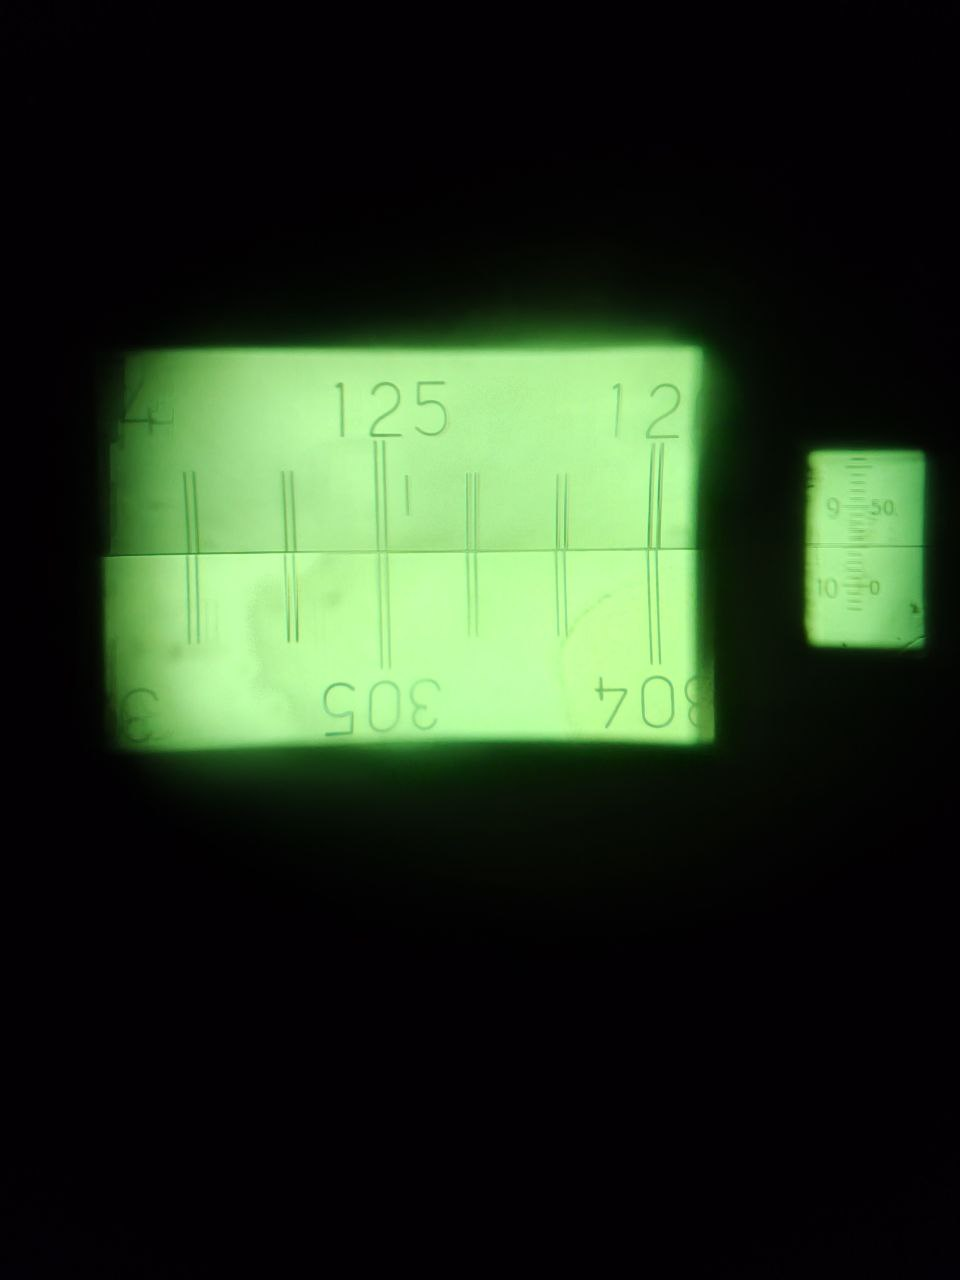
\includegraphics[width=\linewidth]{blue_angle.jpg}
        \caption{Угол спектральной линии света ~492 нм}
        \label{fig:placeholder}
    \end{minipage}
\end{figure}

\begin{table}[H]
\centering
\caption{Зависимость показателя преломления от длины волны}
\begin{tabular}{|c|c|c|}
\hline
№ & $\lambda$, нм & $n$ \\ \hline
1 & 690.7 & 1.6303 \\ \hline
2 & 623.4 & 1.6375 \\ \hline
3 & 579.1 & 1.6440 \\ \hline
4 & 577.0 & 1.6443 \\ \hline
5 & 546.1 & 1.6488 \\ \hline
6 & 491.6 & 1.6597 \\ \hline
7 & 435.8 & 1.6774 \\ \hline
8 & 404.7 & 1.6932 \\ \hline
\end{tabular}
\end{table}

\noindent
Погрешность измерения считаем за $0^\circ0'1''$. При этом погрешность вычисленных $n$ не превышает $8\times10^{-6}$ для любого результата в таблице. \\
\begin{equation}
    \Delta n = \sqrt{\left( \frac{\partial n}{\partial \alpha} \Delta \alpha \right)^2 + \left( \frac{\partial n}{\partial \delta} \Delta \delta \right)^2}
\end{equation}
Теперь построим дисперсионную кривую (Рис. 4). 
\begin{figure}[H]
    \centering
    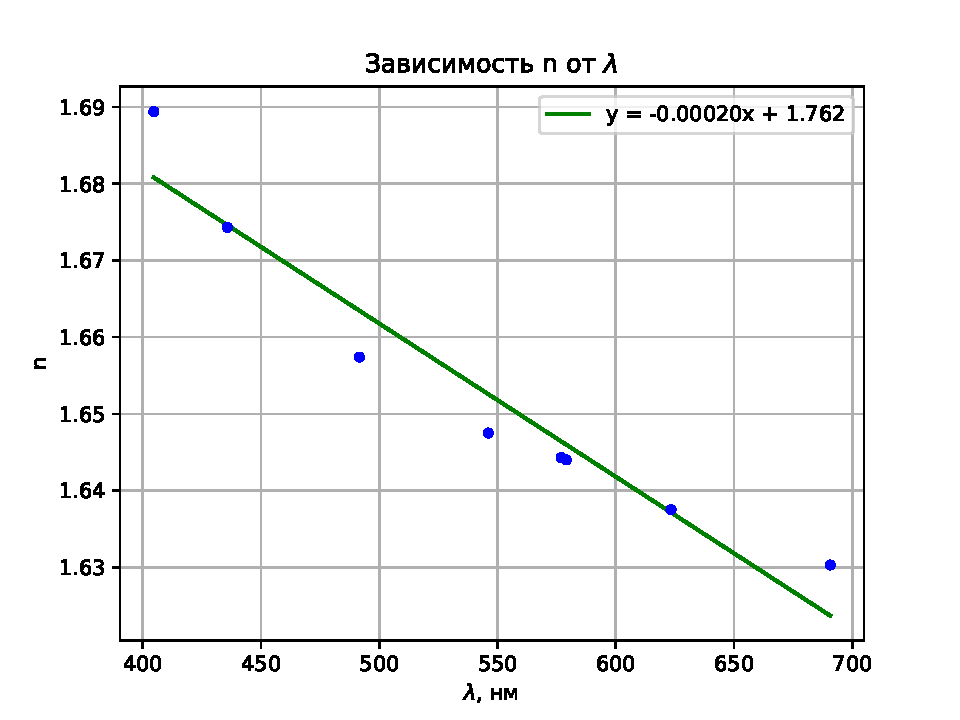
\includegraphics[width=0.75\linewidth]{Зависимость n от lambda.pdf}
    \caption{Дисперсионная кривая}
    \label{fig:placeholder}
\end{figure}

\begin{equation}
{\frac{dn}{d\lambda} \approx -2.0 \cdot 10^{-4}\ \text{нм}^{-1}}.
\end{equation}
Марка стекла в исследуемой призме - ТФ1.
\section*{Выводы}
\begin{itemize}
\item Определен преломляющий угол изучаемой призмы ($\alpha = 62^\circ57'50''$);
\item Найден спектр разложения света ртутной лампы, измерены углы заданных областей (Таблица 1);
\item Определены значения показателей преломления в зависимости от длины волны (Таблица 2), построен график (Рис. 4);
\item По графику рассчитано значение асчитано значение $\frac{dn}{d\lambda} \approx -2.0 \cdot 10^{-4}\ \text{нм}^{-1}$, что соответствует значению для стекла марки ТФ1 ($-1.9 \cdot 10^{-4}\ \text{нм}^{-1}$).
\end{itemize}
\end{document}